\documentclass[twoside]{book}

% Packages required by doxygen
\usepackage{calc}
\usepackage{doxygen}
\usepackage{graphicx}
\usepackage[utf8]{inputenc}
\usepackage{makeidx}
\usepackage{multicol}
\usepackage{multirow}
\usepackage{textcomp}
\usepackage[table]{xcolor}

% Font selection
\usepackage[T1]{fontenc}
\usepackage{mathptmx}
\usepackage[scaled=.90]{helvet}
\usepackage{courier}
\usepackage{amssymb}
\usepackage{sectsty}
\renewcommand{\familydefault}{\sfdefault}
\allsectionsfont{%
  \fontseries{bc}\selectfont%
  \color{darkgray}%
}
\renewcommand{\DoxyLabelFont}{%
  \fontseries{bc}\selectfont%
  \color{darkgray}%
}

% Page & text layout
\usepackage{geometry}
\geometry{%
  a4paper,%
  top=2.5cm,%
  bottom=2.5cm,%
  left=2.5cm,%
  right=2.5cm%
}
\tolerance=750
\hfuzz=15pt
\hbadness=750
\setlength{\emergencystretch}{15pt}
\setlength{\parindent}{0cm}
\setlength{\parskip}{0.2cm}
\makeatletter
\renewcommand{\paragraph}{%
  \@startsection{paragraph}{4}{0ex}{-1.0ex}{1.0ex}{%
    \normalfont\normalsize\bfseries\SS@parafont%
  }%
}
\renewcommand{\subparagraph}{%
  \@startsection{subparagraph}{5}{0ex}{-1.0ex}{1.0ex}{%
    \normalfont\normalsize\bfseries\SS@subparafont%
  }%
}
\makeatother

% Headers & footers
\usepackage{fancyhdr}
\pagestyle{fancyplain}
\fancyhead[LE]{\fancyplain{}{\bfseries\thepage}}
\fancyhead[CE]{\fancyplain{}{}}
\fancyhead[RE]{\fancyplain{}{\bfseries\leftmark}}
\fancyhead[LO]{\fancyplain{}{\bfseries\rightmark}}
\fancyhead[CO]{\fancyplain{}{}}
\fancyhead[RO]{\fancyplain{}{\bfseries\thepage}}
\fancyfoot[LE]{\fancyplain{}{}}
\fancyfoot[CE]{\fancyplain{}{}}
\fancyfoot[RE]{\fancyplain{}{\bfseries\scriptsize Generated on Mon Feb 10 2014 23\-:01\-:04 for The Game by Doxygen }}
\fancyfoot[LO]{\fancyplain{}{\bfseries\scriptsize Generated on Mon Feb 10 2014 23\-:01\-:04 for The Game by Doxygen }}
\fancyfoot[CO]{\fancyplain{}{}}
\fancyfoot[RO]{\fancyplain{}{}}
\renewcommand{\footrulewidth}{0.4pt}
\renewcommand{\chaptermark}[1]{%
  \markboth{#1}{}%
}
\renewcommand{\sectionmark}[1]{%
  \markright{\thesection\ #1}%
}

% Indices & bibliography
\usepackage{natbib}
\usepackage[titles]{tocloft}
\setcounter{tocdepth}{3}
\setcounter{secnumdepth}{5}
\makeindex

% Hyperlinks (required, but should be loaded last)
\usepackage{ifpdf}
\ifpdf
  \usepackage[pdftex,pagebackref=true]{hyperref}
\else
  \usepackage[ps2pdf,pagebackref=true]{hyperref}
\fi
\hypersetup{%
  colorlinks=true,%
  linkcolor=blue,%
  citecolor=blue,%
  unicode%
}

% Custom commands
\newcommand{\clearemptydoublepage}{%
  \newpage{\pagestyle{empty}\cleardoublepage}%
}


%===== C O N T E N T S =====

\begin{document}

% Titlepage & ToC
\hypersetup{pageanchor=false}
\pagenumbering{roman}
\begin{titlepage}
\vspace*{7cm}
\begin{center}%
{\Large The Game }\\
\vspace*{1cm}
{\large Generated by Doxygen 1.8.6}\\
\vspace*{0.5cm}
{\small Mon Feb 10 2014 23:01:04}\\
\end{center}
\end{titlepage}
\clearemptydoublepage
\tableofcontents
\clearemptydoublepage
\pagenumbering{arabic}
\hypersetup{pageanchor=true}

%--- Begin generated contents ---
\chapter{Hierarchical Index}
\section{Class Hierarchy}
This inheritance list is sorted roughly, but not completely, alphabetically\-:\begin{DoxyCompactList}
\item \contentsline{section}{game}{\pageref{classgame}}{}
\item Sprite\begin{DoxyCompactList}
\item \contentsline{section}{bounce\-Ball}{\pageref{classbounce_ball}}{}
\item \contentsline{section}{box}{\pageref{classbox}}{}
\begin{DoxyCompactList}
\item \contentsline{section}{steel\-Box}{\pageref{classsteel_box}}{}
\end{DoxyCompactList}
\item \contentsline{section}{gui}{\pageref{classgui}}{}
\item \contentsline{section}{player}{\pageref{classplayer}}{}
\end{DoxyCompactList}
\end{DoxyCompactList}

\chapter{Class Index}
\section{Class List}
Here are the classes, structs, unions and interfaces with brief descriptions\-:\begin{DoxyCompactList}
\item\contentsline{section}{\hyperlink{classbounce_ball}{bounce\-Ball} }{\pageref{classbounce_ball}}{}
\item\contentsline{section}{\hyperlink{classbox}{box} }{\pageref{classbox}}{}
\item\contentsline{section}{\hyperlink{classgame}{game} }{\pageref{classgame}}{}
\item\contentsline{section}{\hyperlink{classgui}{gui} }{\pageref{classgui}}{}
\item\contentsline{section}{\hyperlink{classplayer}{player} }{\pageref{classplayer}}{}
\item\contentsline{section}{\hyperlink{classsteel_box}{steel\-Box} }{\pageref{classsteel_box}}{}
\end{DoxyCompactList}

\chapter{File Index}
\section{File List}
Here is a list of all files with brief descriptions\-:\begin{DoxyCompactList}
\item\contentsline{section}{/home/mejan/\-Documents/skola/\-Cvilingjör\-I\-Datateknik/\-H\-T-\/13/\-Programerings\-\_\-metodiken/\-Projekt/\hyperlink{bounceball_8cpp}{bounceball.\-cpp} }{\pageref{bounceball_8cpp}}{}
\item\contentsline{section}{/home/mejan/\-Documents/skola/\-Cvilingjör\-I\-Datateknik/\-H\-T-\/13/\-Programerings\-\_\-metodiken/\-Projekt/\hyperlink{bounceball_8h}{bounceball.\-h} }{\pageref{bounceball_8h}}{}
\item\contentsline{section}{/home/mejan/\-Documents/skola/\-Cvilingjör\-I\-Datateknik/\-H\-T-\/13/\-Programerings\-\_\-metodiken/\-Projekt/\hyperlink{box_8cpp}{box.\-cpp} }{\pageref{box_8cpp}}{}
\item\contentsline{section}{/home/mejan/\-Documents/skola/\-Cvilingjör\-I\-Datateknik/\-H\-T-\/13/\-Programerings\-\_\-metodiken/\-Projekt/\hyperlink{box_8h}{box.\-h} }{\pageref{box_8h}}{}
\item\contentsline{section}{/home/mejan/\-Documents/skola/\-Cvilingjör\-I\-Datateknik/\-H\-T-\/13/\-Programerings\-\_\-metodiken/\-Projekt/\hyperlink{game_8cpp}{game.\-cpp} }{\pageref{game_8cpp}}{}
\item\contentsline{section}{/home/mejan/\-Documents/skola/\-Cvilingjör\-I\-Datateknik/\-H\-T-\/13/\-Programerings\-\_\-metodiken/\-Projekt/\hyperlink{game_8h}{game.\-h} }{\pageref{game_8h}}{}
\item\contentsline{section}{/home/mejan/\-Documents/skola/\-Cvilingjör\-I\-Datateknik/\-H\-T-\/13/\-Programerings\-\_\-metodiken/\-Projekt/\hyperlink{gui_8cpp}{gui.\-cpp} }{\pageref{gui_8cpp}}{}
\item\contentsline{section}{/home/mejan/\-Documents/skola/\-Cvilingjör\-I\-Datateknik/\-H\-T-\/13/\-Programerings\-\_\-metodiken/\-Projekt/\hyperlink{gui_8h}{gui.\-h} }{\pageref{gui_8h}}{}
\item\contentsline{section}{/home/mejan/\-Documents/skola/\-Cvilingjör\-I\-Datateknik/\-H\-T-\/13/\-Programerings\-\_\-metodiken/\-Projekt/\hyperlink{main_8cpp}{main.\-cpp} }{\pageref{main_8cpp}}{}
\item\contentsline{section}{/home/mejan/\-Documents/skola/\-Cvilingjör\-I\-Datateknik/\-H\-T-\/13/\-Programerings\-\_\-metodiken/\-Projekt/\hyperlink{player_8cpp}{player.\-cpp} }{\pageref{player_8cpp}}{}
\item\contentsline{section}{/home/mejan/\-Documents/skola/\-Cvilingjör\-I\-Datateknik/\-H\-T-\/13/\-Programerings\-\_\-metodiken/\-Projekt/\hyperlink{player_8h}{player.\-h} }{\pageref{player_8h}}{}
\item\contentsline{section}{/home/mejan/\-Documents/skola/\-Cvilingjör\-I\-Datateknik/\-H\-T-\/13/\-Programerings\-\_\-metodiken/\-Projekt/\hyperlink{steel_box_8cpp}{steel\-Box.\-cpp} }{\pageref{steel_box_8cpp}}{}
\item\contentsline{section}{/home/mejan/\-Documents/skola/\-Cvilingjör\-I\-Datateknik/\-H\-T-\/13/\-Programerings\-\_\-metodiken/\-Projekt/\hyperlink{steel_box_8h}{steel\-Box.\-h} }{\pageref{steel_box_8h}}{}
\end{DoxyCompactList}

\chapter{Class Documentation}
\hypertarget{classbounce_ball}{\section{bounce\-Ball Class Reference}
\label{classbounce_ball}\index{bounce\-Ball@{bounce\-Ball}}
}


{\ttfamily \#include $<$bounceball.\-h$>$}

Inheritance diagram for bounce\-Ball\-:\begin{figure}[H]
\begin{center}
\leavevmode
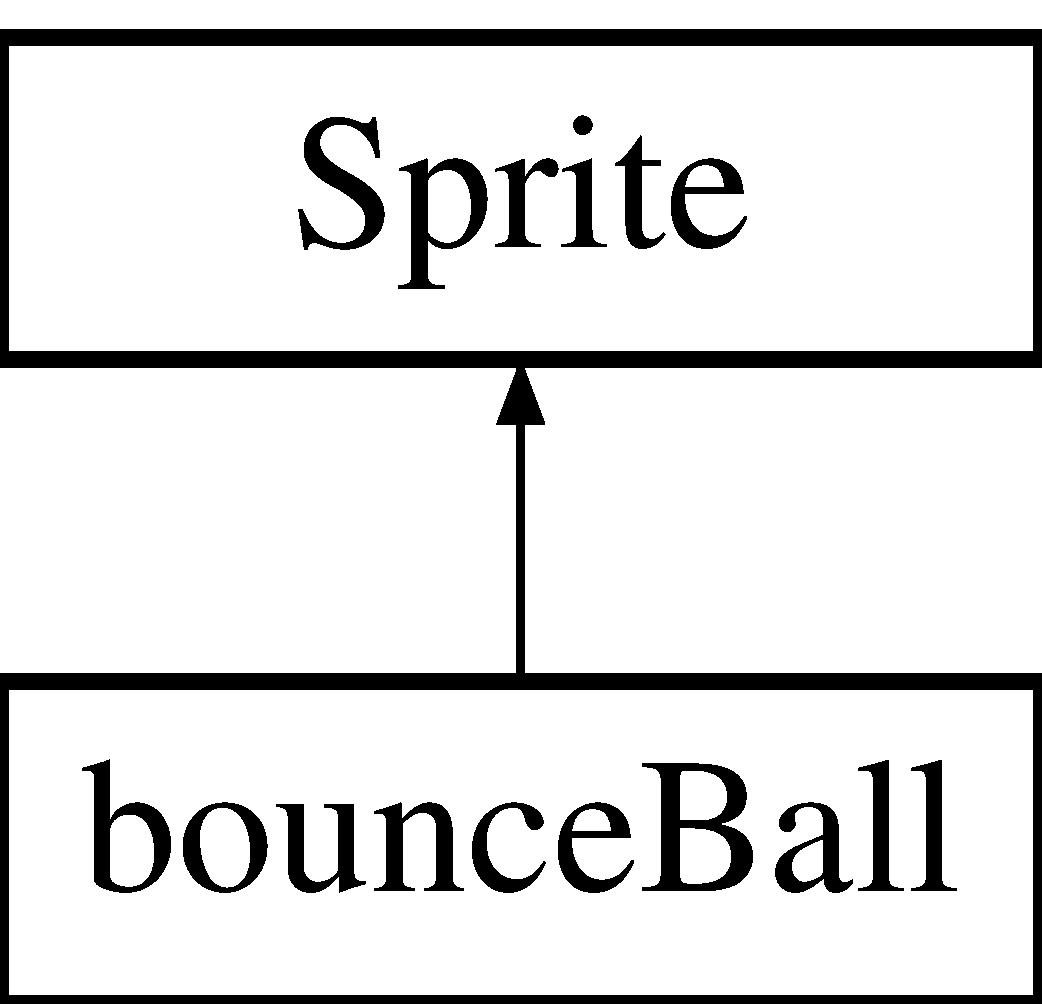
\includegraphics[height=2.000000cm]{classbounce_ball}
\end{center}
\end{figure}
\subsection*{Public Member Functions}
\begin{DoxyCompactItemize}
\item 
\hyperlink{classbounce_ball_ab9cd9e9e07b75288688ddf48e8805808}{bounce\-Ball} ()
\item 
\hyperlink{classbounce_ball_a5aade551a140ca729b82db53a71923ea}{$\sim$bounce\-Ball} ()
\item 
void \hyperlink{classbounce_ball_a05e818abbd26e5f24f08604557b99be2}{movement\-Of\-Ball} (sf\-::\-Int32 \&update)
\item 
bool \hyperlink{classbounce_ball_aef61d98587fe7ac412dee9578dbad59d}{check\-If\-Dead} ()
\item 
void \hyperlink{classbounce_ball_ae23ce7e3294786a71ab6975162d3e08a}{set\-Ball\-Direction\-Y} (float y)
\item 
void \hyperlink{classbounce_ball_a81160a8f16a17df7906fbf624f62f857}{set\-Ball\-Direction\-X} (float x)
\item 
double \hyperlink{classbounce_ball_ac7d3e884d8b6d1f0f902dcf5be3a3890}{get\-Ball\-Direction\-Y} () const 
\item 
double \hyperlink{classbounce_ball_a5868831d08186838d6e21a35c8f733ad}{get\-Ball\-Direction\-X} () const 
\item 
bool \hyperlink{classbounce_ball_a3eb081b76ad67cc68759d3149e334b54}{shall\-Collide\-With} (sf\-::\-Sprite \&s, sf\-::\-Int32 update)
\end{DoxyCompactItemize}


\subsection{Detailed Description}
\hyperlink{classbounce_ball}{bounce\-Ball} class the ball movement functions.

this is the class for a ball that can change the direktion. and is supose to always be moving. 

Definition at line 14 of file bounceball.\-h.



\subsection{Constructor \& Destructor Documentation}
\hypertarget{classbounce_ball_ab9cd9e9e07b75288688ddf48e8805808}{\index{bounce\-Ball@{bounce\-Ball}!bounce\-Ball@{bounce\-Ball}}
\index{bounce\-Ball@{bounce\-Ball}!bounceBall@{bounce\-Ball}}
\subsubsection[{bounce\-Ball}]{\setlength{\rightskip}{0pt plus 5cm}bounce\-Ball\-::bounce\-Ball (
\begin{DoxyParamCaption}
{}
\end{DoxyParamCaption}
)}}\label{classbounce_ball_ab9cd9e9e07b75288688ddf48e8805808}
Constructor that loads texture to the ball set it's origin and start position. and randomly chose 1 of four start directions. 

Definition at line 5 of file bounceball.\-cpp.

\hypertarget{classbounce_ball_a5aade551a140ca729b82db53a71923ea}{\index{bounce\-Ball@{bounce\-Ball}!$\sim$bounce\-Ball@{$\sim$bounce\-Ball}}
\index{$\sim$bounce\-Ball@{$\sim$bounce\-Ball}!bounceBall@{bounce\-Ball}}
\subsubsection[{$\sim$bounce\-Ball}]{\setlength{\rightskip}{0pt plus 5cm}bounce\-Ball\-::$\sim$bounce\-Ball (
\begin{DoxyParamCaption}
{}
\end{DoxyParamCaption}
)}}\label{classbounce_ball_a5aade551a140ca729b82db53a71923ea}
do not have a function just there for show. 

Definition at line 28 of file bounceball.\-cpp.



\subsection{Member Function Documentation}
\hypertarget{classbounce_ball_aef61d98587fe7ac412dee9578dbad59d}{\index{bounce\-Ball@{bounce\-Ball}!check\-If\-Dead@{check\-If\-Dead}}
\index{check\-If\-Dead@{check\-If\-Dead}!bounceBall@{bounce\-Ball}}
\subsubsection[{check\-If\-Dead}]{\setlength{\rightskip}{0pt plus 5cm}bool bounce\-Ball\-::check\-If\-Dead (
\begin{DoxyParamCaption}
{}
\end{DoxyParamCaption}
)}}\label{classbounce_ball_aef61d98587fe7ac412dee9578dbad59d}
returns that the ball is dead if it's under the window. returns true if ball 800 px from window top. returns false if above. 

Definition at line 34 of file bounceball.\-cpp.

\hypertarget{classbounce_ball_a5868831d08186838d6e21a35c8f733ad}{\index{bounce\-Ball@{bounce\-Ball}!get\-Ball\-Direction\-X@{get\-Ball\-Direction\-X}}
\index{get\-Ball\-Direction\-X@{get\-Ball\-Direction\-X}!bounceBall@{bounce\-Ball}}
\subsubsection[{get\-Ball\-Direction\-X}]{\setlength{\rightskip}{0pt plus 5cm}double bounce\-Ball\-::get\-Ball\-Direction\-X (
\begin{DoxyParamCaption}
{}
\end{DoxyParamCaption}
) const}}\label{classbounce_ball_a5868831d08186838d6e21a35c8f733ad}
returns the X axel direction/speed. 

Definition at line 55 of file bounceball.\-cpp.

\hypertarget{classbounce_ball_ac7d3e884d8b6d1f0f902dcf5be3a3890}{\index{bounce\-Ball@{bounce\-Ball}!get\-Ball\-Direction\-Y@{get\-Ball\-Direction\-Y}}
\index{get\-Ball\-Direction\-Y@{get\-Ball\-Direction\-Y}!bounceBall@{bounce\-Ball}}
\subsubsection[{get\-Ball\-Direction\-Y}]{\setlength{\rightskip}{0pt plus 5cm}double bounce\-Ball\-::get\-Ball\-Direction\-Y (
\begin{DoxyParamCaption}
{}
\end{DoxyParamCaption}
) const}}\label{classbounce_ball_ac7d3e884d8b6d1f0f902dcf5be3a3890}
retruns the Y axel direction/speed. 

Definition at line 51 of file bounceball.\-cpp.

\hypertarget{classbounce_ball_a05e818abbd26e5f24f08604557b99be2}{\index{bounce\-Ball@{bounce\-Ball}!movement\-Of\-Ball@{movement\-Of\-Ball}}
\index{movement\-Of\-Ball@{movement\-Of\-Ball}!bounceBall@{bounce\-Ball}}
\subsubsection[{movement\-Of\-Ball}]{\setlength{\rightskip}{0pt plus 5cm}void bounce\-Ball\-::movement\-Of\-Ball (
\begin{DoxyParamCaption}
\item[{sf\-::\-Int32 \&}]{update}
\end{DoxyParamCaption}
)}}\label{classbounce_ball_a05e818abbd26e5f24f08604557b99be2}
moves the ball, with a clock to make it smother. 

Definition at line 30 of file bounceball.\-cpp.

\hypertarget{classbounce_ball_a81160a8f16a17df7906fbf624f62f857}{\index{bounce\-Ball@{bounce\-Ball}!set\-Ball\-Direction\-X@{set\-Ball\-Direction\-X}}
\index{set\-Ball\-Direction\-X@{set\-Ball\-Direction\-X}!bounceBall@{bounce\-Ball}}
\subsubsection[{set\-Ball\-Direction\-X}]{\setlength{\rightskip}{0pt plus 5cm}void bounce\-Ball\-::set\-Ball\-Direction\-X (
\begin{DoxyParamCaption}
\item[{float}]{x}
\end{DoxyParamCaption}
)}}\label{classbounce_ball_a81160a8f16a17df7906fbf624f62f857}
change the X axel direction/speed of ball with this function Input float. 

Definition at line 47 of file bounceball.\-cpp.

\hypertarget{classbounce_ball_ae23ce7e3294786a71ab6975162d3e08a}{\index{bounce\-Ball@{bounce\-Ball}!set\-Ball\-Direction\-Y@{set\-Ball\-Direction\-Y}}
\index{set\-Ball\-Direction\-Y@{set\-Ball\-Direction\-Y}!bounceBall@{bounce\-Ball}}
\subsubsection[{set\-Ball\-Direction\-Y}]{\setlength{\rightskip}{0pt plus 5cm}void bounce\-Ball\-::set\-Ball\-Direction\-Y (
\begin{DoxyParamCaption}
\item[{float}]{y}
\end{DoxyParamCaption}
)}}\label{classbounce_ball_ae23ce7e3294786a71ab6975162d3e08a}
change the Y axel direction/speed of ball with this function Input float. 

Definition at line 43 of file bounceball.\-cpp.

\hypertarget{classbounce_ball_a3eb081b76ad67cc68759d3149e334b54}{\index{bounce\-Ball@{bounce\-Ball}!shall\-Collide\-With@{shall\-Collide\-With}}
\index{shall\-Collide\-With@{shall\-Collide\-With}!bounceBall@{bounce\-Ball}}
\subsubsection[{shall\-Collide\-With}]{\setlength{\rightskip}{0pt plus 5cm}bool bounce\-Ball\-::shall\-Collide\-With (
\begin{DoxyParamCaption}
\item[{sf\-::\-Sprite \&}]{s, }
\item[{sf\-::\-Int32}]{update}
\end{DoxyParamCaption}
)}}\label{classbounce_ball_a3eb081b76ad67cc68759d3149e334b54}
Input sprite, if ball collide with sprite it will bounce on it. and return true. else return false and continue in old direction/speed.

checks where and how the balls collides with a other object and desides the new direction/speed that it should have. 

Definition at line 62 of file bounceball.\-cpp.



The documentation for this class was generated from the following files\-:\begin{DoxyCompactItemize}
\item 
/home/mejan/\-Documents/skola/\-Cvilingjör\-I\-Datateknik/\-H\-T-\/13/\-Programerings\-\_\-metodiken/\-Projekt/\hyperlink{bounceball_8h}{bounceball.\-h}\item 
/home/mejan/\-Documents/skola/\-Cvilingjör\-I\-Datateknik/\-H\-T-\/13/\-Programerings\-\_\-metodiken/\-Projekt/\hyperlink{bounceball_8cpp}{bounceball.\-cpp}\end{DoxyCompactItemize}

\hypertarget{classbox}{\section{box Class Reference}
\label{classbox}\index{box@{box}}
}


{\ttfamily \#include $<$box.\-h$>$}

Inheritance diagram for box\-:\begin{figure}[H]
\begin{center}
\leavevmode
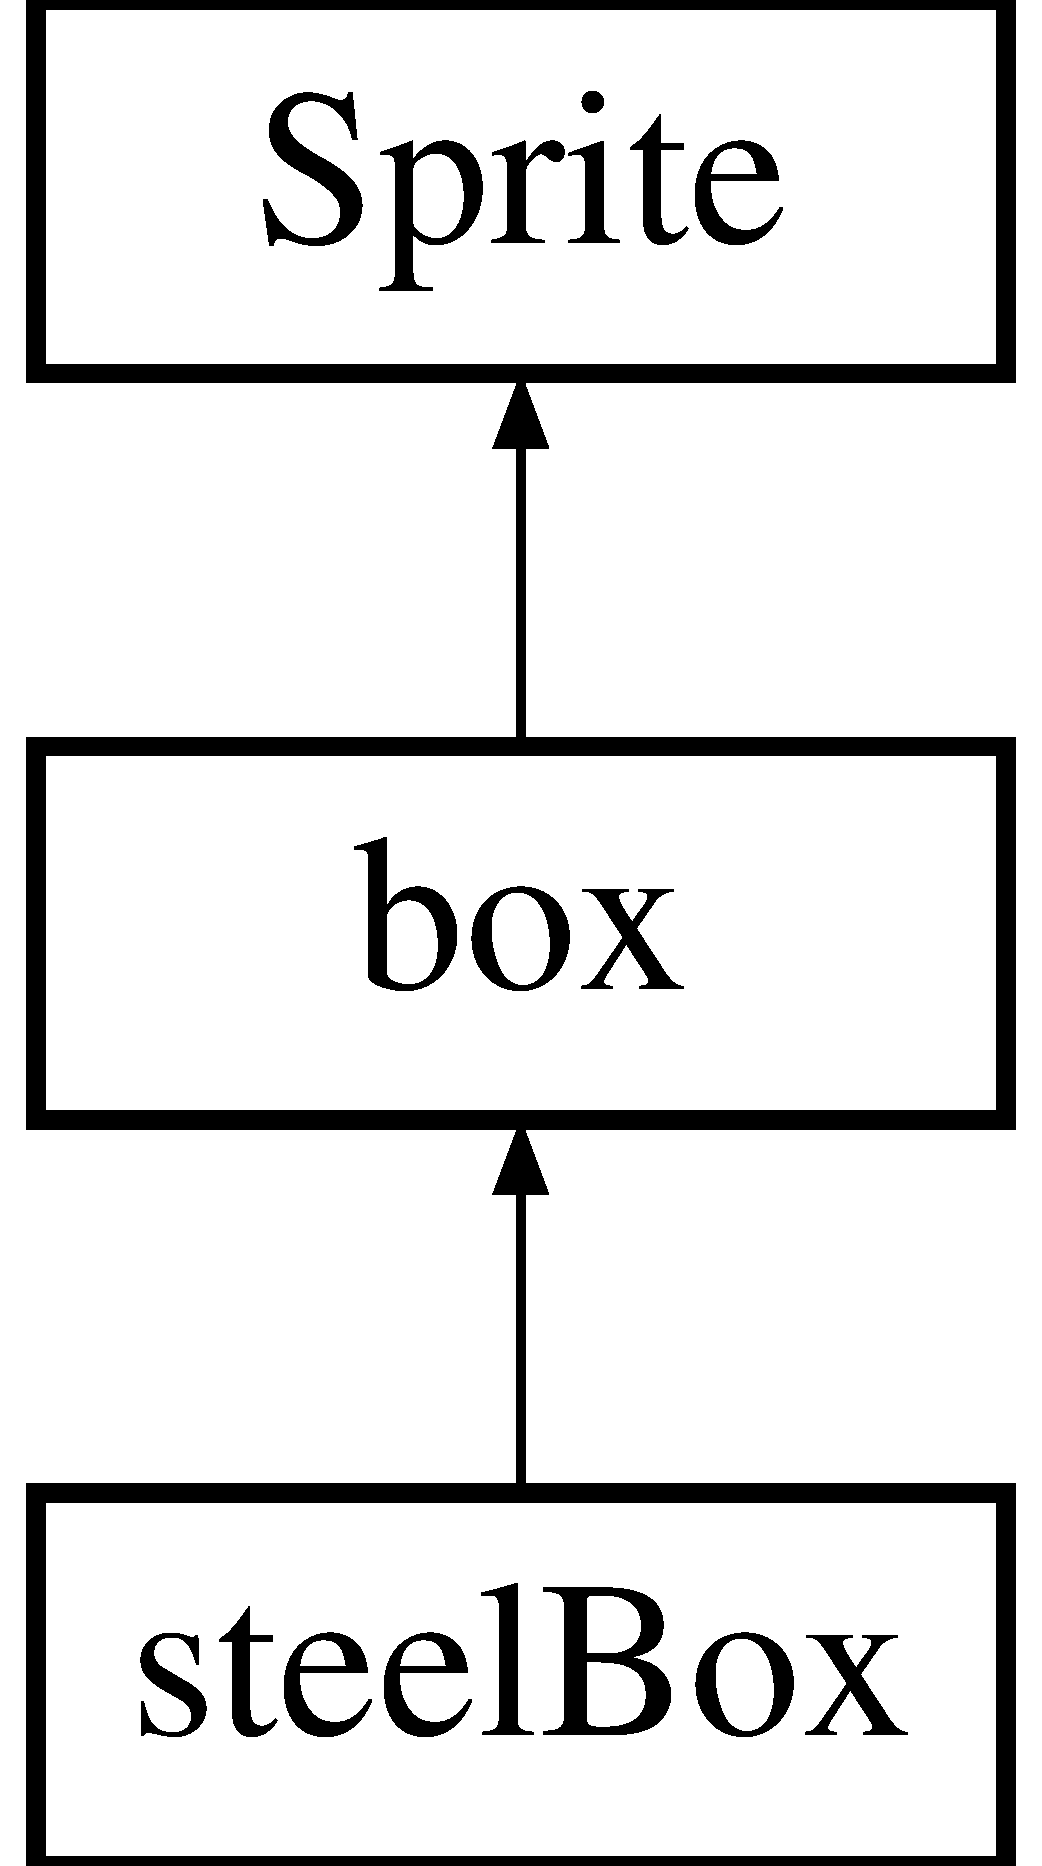
\includegraphics[height=3.000000cm]{classbox}
\end{center}
\end{figure}
\subsection*{Public Member Functions}
\begin{DoxyCompactItemize}
\item 
\hyperlink{classbox_a1ca802dd9502ab576e4786c06325fd94}{box} ()
\item 
\hyperlink{classbox_a4a171e8fb066fd52707f5277042c1f6b}{box} (std\-::string txt, int h)
\item 
\hyperlink{classbox_ad9af3cd34d85201cce706f00dab584c9}{$\sim$box} ()
\item 
int \hyperlink{classbox_ae3da136dd05139a6ab352639b290f219}{get\-Life} () const 
\item 
void \hyperlink{classbox_ac425fbd403147efa5e0f07f6d9396df6}{lose\-Life} ()
\end{DoxyCompactItemize}


\subsection{Detailed Description}
the box object

this is the class the player should destroy. 

Definition at line 14 of file box.\-h.



\subsection{Constructor \& Destructor Documentation}
\hypertarget{classbox_a1ca802dd9502ab576e4786c06325fd94}{\index{box@{box}!box@{box}}
\index{box@{box}!box@{box}}
\subsubsection[{box}]{\setlength{\rightskip}{0pt plus 5cm}box\-::box (
\begin{DoxyParamCaption}
{}
\end{DoxyParamCaption}
)}}\label{classbox_a1ca802dd9502ab576e4786c06325fd94}
default constructor loads a texture and sets the origin. sets health to 1. 

Definition at line 3 of file box.\-cpp.

\hypertarget{classbox_a4a171e8fb066fd52707f5277042c1f6b}{\index{box@{box}!box@{box}}
\index{box@{box}!box@{box}}
\subsubsection[{box}]{\setlength{\rightskip}{0pt plus 5cm}box\-::box (
\begin{DoxyParamCaption}
\item[{std\-::string}]{txt, }
\item[{int}]{h}
\end{DoxyParamCaption}
)}}\label{classbox_a4a171e8fb066fd52707f5277042c1f6b}
constructor that takes input as where it should load the texture from and how mutch health the box should have. 

Definition at line 13 of file box.\-cpp.

\hypertarget{classbox_ad9af3cd34d85201cce706f00dab584c9}{\index{box@{box}!$\sim$box@{$\sim$box}}
\index{$\sim$box@{$\sim$box}!box@{box}}
\subsubsection[{$\sim$box}]{\setlength{\rightskip}{0pt plus 5cm}box\-::$\sim$box (
\begin{DoxyParamCaption}
{}
\end{DoxyParamCaption}
)}}\label{classbox_ad9af3cd34d85201cce706f00dab584c9}


Definition at line 22 of file box.\-cpp.



\subsection{Member Function Documentation}
\hypertarget{classbox_ae3da136dd05139a6ab352639b290f219}{\index{box@{box}!get\-Life@{get\-Life}}
\index{get\-Life@{get\-Life}!box@{box}}
\subsubsection[{get\-Life}]{\setlength{\rightskip}{0pt plus 5cm}int box\-::get\-Life (
\begin{DoxyParamCaption}
{}
\end{DoxyParamCaption}
) const}}\label{classbox_ae3da136dd05139a6ab352639b290f219}
returns the current health of the box. 

Definition at line 25 of file box.\-cpp.

\hypertarget{classbox_ac425fbd403147efa5e0f07f6d9396df6}{\index{box@{box}!lose\-Life@{lose\-Life}}
\index{lose\-Life@{lose\-Life}!box@{box}}
\subsubsection[{lose\-Life}]{\setlength{\rightskip}{0pt plus 5cm}void box\-::lose\-Life (
\begin{DoxyParamCaption}
{}
\end{DoxyParamCaption}
)}}\label{classbox_ac425fbd403147efa5e0f07f6d9396df6}
lessens the health of the box with 1. 

Definition at line 30 of file box.\-cpp.



The documentation for this class was generated from the following files\-:\begin{DoxyCompactItemize}
\item 
/home/mejan/\-Documents/skola/\-Cvilingjör\-I\-Datateknik/\-H\-T-\/13/\-Programerings\-\_\-metodiken/\-Projekt/\hyperlink{box_8h}{box.\-h}\item 
/home/mejan/\-Documents/skola/\-Cvilingjör\-I\-Datateknik/\-H\-T-\/13/\-Programerings\-\_\-metodiken/\-Projekt/\hyperlink{box_8cpp}{box.\-cpp}\end{DoxyCompactItemize}

\hypertarget{classgame}{\section{game Class Reference}
\label{classgame}\index{game@{game}}
}


{\ttfamily \#include $<$game.\-h$>$}

\subsection*{Public Member Functions}
\begin{DoxyCompactItemize}
\item 
\hyperlink{classgame_ad9c102127b5038f880067ad6c9198d38}{game} ()
\item 
\hyperlink{classgame_ae87abd20c4d8a7906fa48e690a5f1d07}{$\sim$game} ()
\item 
void \hyperlink{classgame_a71335d048da0ecac0ce4935697c0a9e9}{execute} ()
\end{DoxyCompactItemize}


\subsection{Detailed Description}
The Game class, has all the objects and will check events, updates and draw/render for displaying the game for users.

This class uses the other classes by dynamic memory, in the event the class checks for user input and set varibles accordently. Update will update the new positions of object and check if collides with each other. render is used to render all the dynamic objects to be displayed in the window. 

Definition at line 25 of file game.\-h.



\subsection{Constructor \& Destructor Documentation}
\hypertarget{classgame_ad9c102127b5038f880067ad6c9198d38}{\index{game@{game}!game@{game}}
\index{game@{game}!game@{game}}
\subsubsection[{game}]{\setlength{\rightskip}{0pt plus 5cm}game\-::game (
\begin{DoxyParamCaption}
{}
\end{DoxyParamCaption}
)}}\label{classgame_ad9c102127b5038f880067ad6c9198d38}
Construtctor for the game set up the window size and titel, the key repeat disable. sets fps limit at 60 fps. calls a private function called set\-Up\-Walls that prepare the walls that the ball bounce on. it calls set\-Up\-Text, is there to prepare all the texts object this class has. Direct new gui to the meny pointer. It calls a private member function called new\-Game witch alocate dynamicly all the objects in the game. then it calls the public member function execute. 

Definition at line 3 of file game.\-cpp.

\hypertarget{classgame_ae87abd20c4d8a7906fa48e690a5f1d07}{\index{game@{game}!$\sim$game@{$\sim$game}}
\index{$\sim$game@{$\sim$game}!game@{game}}
\subsubsection[{$\sim$game}]{\setlength{\rightskip}{0pt plus 5cm}game\-::$\sim$game (
\begin{DoxyParamCaption}
{}
\end{DoxyParamCaption}
)}}\label{classgame_ae87abd20c4d8a7906fa48e690a5f1d07}
distructor just delete all the allocated memeory. 

Definition at line 17 of file game.\-cpp.



\subsection{Member Function Documentation}
\hypertarget{classgame_a71335d048da0ecac0ce4935697c0a9e9}{\index{game@{game}!execute@{execute}}
\index{execute@{execute}!game@{game}}
\subsubsection[{execute}]{\setlength{\rightskip}{0pt plus 5cm}void game\-::execute (
\begin{DoxyParamCaption}
{}
\end{DoxyParamCaption}
)}}\label{classgame_a71335d048da0ecac0ce4935697c0a9e9}
Execute has som diffrent clock/timer to controll the fps will be right.

The main thing about the member function is that it's a while that will continue while window is open, and it checks for events of users/program these events are trigger diffrent viribles to change value.

Then it will call update, update changes the possistions and looks for collitions between objects and check if the that object should be removed.

Then the private memberfunction render is called where it clears the screen and then draws/render the objects positions and display it in the widniow. 

Definition at line 24 of file game.\-cpp.



The documentation for this class was generated from the following files\-:\begin{DoxyCompactItemize}
\item 
/home/mejan/\-Documents/skola/\-Cvilingjör\-I\-Datateknik/\-H\-T-\/13/\-Programerings\-\_\-metodiken/\-Projekt/\hyperlink{game_8h}{game.\-h}\item 
/home/mejan/\-Documents/skola/\-Cvilingjör\-I\-Datateknik/\-H\-T-\/13/\-Programerings\-\_\-metodiken/\-Projekt/\hyperlink{game_8cpp}{game.\-cpp}\end{DoxyCompactItemize}

\hypertarget{classgui}{\section{gui Class Reference}
\label{classgui}\index{gui@{gui}}
}


{\ttfamily \#include $<$gui.\-h$>$}

Inheritance diagram for gui\-:\begin{figure}[H]
\begin{center}
\leavevmode
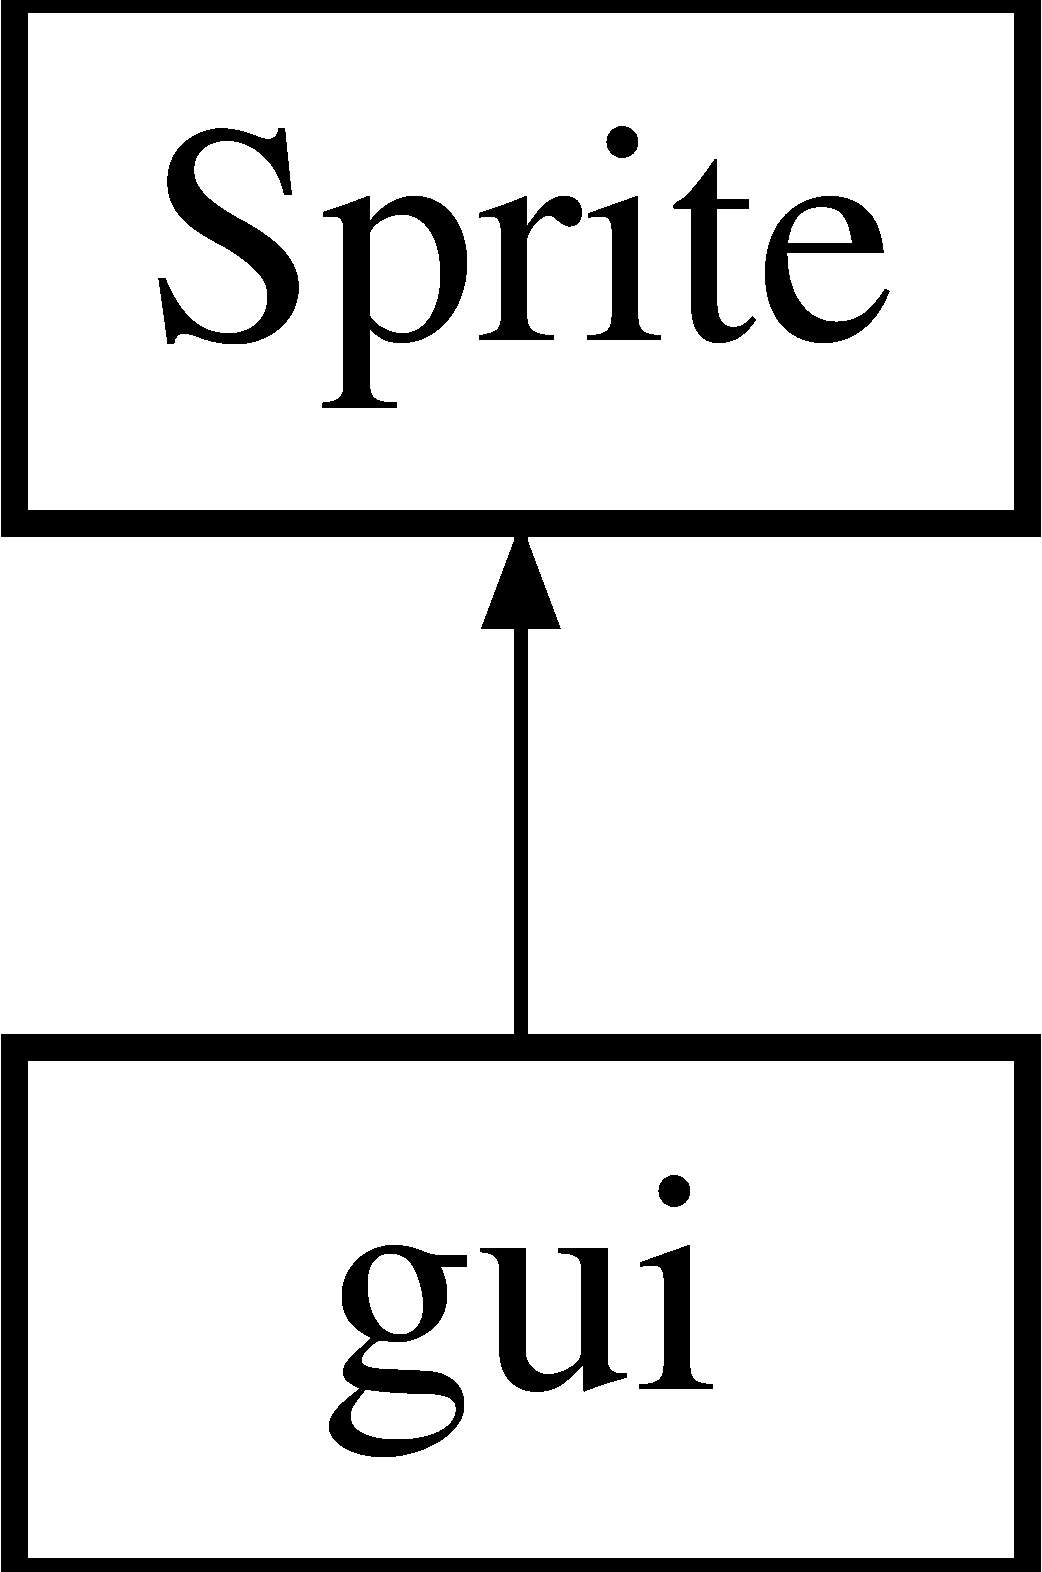
\includegraphics[height=2.000000cm]{classgui}
\end{center}
\end{figure}
\subsection*{Public Member Functions}
\begin{DoxyCompactItemize}
\item 
\hyperlink{classgui_a83e2c722e7fec575b45b9cb33b73607d}{gui} ()
\item 
\hyperlink{classgui_aec3eac5e4971812949be5e1a8a82ce55}{$\sim$gui} ()
\item 
void \hyperlink{classgui_adb0d03c56fce76b17a4884da45819525}{gui\-Update} ()
\item 
void \hyperlink{classgui_af6e2c9f41dae730e0b981ede035ca17c}{set\-Markted\-On\-Meny} (bool markted)
\item 
void \hyperlink{classgui_ab9d74152a7940692cb0c7a6edae1a9c3}{set\-Choice\-Done} ()
\item 
void \hyperlink{classgui_ad0d717e33022d183e43c88271ca5223e}{game\-Over} (sf\-::\-Int32 \&update)
\item 
void \hyperlink{classgui_ae28760870545c851ce09dfc691a4cd48}{winner} (sf\-::\-Int32 \&update)
\item 
bool \hyperlink{classgui_a7740e38a83ea37765bc62d3b18e9a944}{get\-Play} ()
\item 
bool \hyperlink{classgui_a7366788ae4d6c53f8a9474482d20490a}{get\-Show\-Meny} () const 
\item 
sf\-::\-Text \hyperlink{classgui_a9ff3aea558d1d738b33af5faece0c278}{get\-Start} ()
\item 
sf\-::\-Text \hyperlink{classgui_ada8b28974e6d5d6f6419f9d9aa8c3324}{get\-Quit} ()
\item 
sf\-::\-Text \hyperlink{classgui_a01078d72a91a9c5d224f3069a16aaf49}{get\-Game\-Over} ()
\item 
sf\-::\-Text \hyperlink{classgui_ad8947f61e2f74be47ef6c729fcb7352c}{get\-Win} ()
\item 
void \hyperlink{classgui_a106730791e450bc2a0d1022c3b28089e}{new\-Game\-Over} ()
\item 
void \hyperlink{classgui_ade8187f38b25d416a36cea7385c29cc6}{new\-Win} ()
\end{DoxyCompactItemize}


\subsection{Detailed Description}


Definition at line 7 of file gui.\-h.



\subsection{Constructor \& Destructor Documentation}
\hypertarget{classgui_a83e2c722e7fec575b45b9cb33b73607d}{\index{gui@{gui}!gui@{gui}}
\index{gui@{gui}!gui@{gui}}
\subsubsection[{gui}]{\setlength{\rightskip}{0pt plus 5cm}gui\-::gui (
\begin{DoxyParamCaption}
{}
\end{DoxyParamCaption}
)}}\label{classgui_a83e2c722e7fec575b45b9cb33b73607d}
default construtor for the gui.

loads background texture. set showmeny to true. set the meny to mark the start text. setting up the diffrent text objects. and sets the moving speed and direction of gameover and winning text objects. 

Definition at line 3 of file gui.\-cpp.

\hypertarget{classgui_aec3eac5e4971812949be5e1a8a82ce55}{\index{gui@{gui}!$\sim$gui@{$\sim$gui}}
\index{$\sim$gui@{$\sim$gui}!gui@{gui}}
\subsubsection[{$\sim$gui}]{\setlength{\rightskip}{0pt plus 5cm}gui\-::$\sim$gui (
\begin{DoxyParamCaption}
{}
\end{DoxyParamCaption}
)}}\label{classgui_aec3eac5e4971812949be5e1a8a82ce55}


Definition at line 44 of file gui.\-cpp.



\subsection{Member Function Documentation}
\hypertarget{classgui_ad0d717e33022d183e43c88271ca5223e}{\index{gui@{gui}!game\-Over@{game\-Over}}
\index{game\-Over@{game\-Over}!gui@{gui}}
\subsubsection[{game\-Over}]{\setlength{\rightskip}{0pt plus 5cm}void gui\-::game\-Over (
\begin{DoxyParamCaption}
\item[{sf\-::\-Int32 \&}]{update}
\end{DoxyParamCaption}
)}}\label{classgui_ad0d717e33022d183e43c88271ca5223e}
moves the gameover text from roof to middel when moved to the middel it then sets that the meny should be shown again. and set that user made choice to false again. when the text is in the middel it sets showmeny to true. 

Definition at line 66 of file gui.\-cpp.

\hypertarget{classgui_a01078d72a91a9c5d224f3069a16aaf49}{\index{gui@{gui}!get\-Game\-Over@{get\-Game\-Over}}
\index{get\-Game\-Over@{get\-Game\-Over}!gui@{gui}}
\subsubsection[{get\-Game\-Over}]{\setlength{\rightskip}{0pt plus 5cm}sf\-::\-Text gui\-::get\-Game\-Over (
\begin{DoxyParamCaption}
{}
\end{DoxyParamCaption}
)}}\label{classgui_a01078d72a91a9c5d224f3069a16aaf49}
returns text object Game\-Over 

Definition at line 115 of file gui.\-cpp.

\hypertarget{classgui_a7740e38a83ea37765bc62d3b18e9a944}{\index{gui@{gui}!get\-Play@{get\-Play}}
\index{get\-Play@{get\-Play}!gui@{gui}}
\subsubsection[{get\-Play}]{\setlength{\rightskip}{0pt plus 5cm}bool gui\-::get\-Play (
\begin{DoxyParamCaption}
{}
\end{DoxyParamCaption}
)}}\label{classgui_a7740e38a83ea37765bc62d3b18e9a944}
returns a bool value true aslong as quit Text object in gui is the choice. 

Definition at line 86 of file gui.\-cpp.

\hypertarget{classgui_ada8b28974e6d5d6f6419f9d9aa8c3324}{\index{gui@{gui}!get\-Quit@{get\-Quit}}
\index{get\-Quit@{get\-Quit}!gui@{gui}}
\subsubsection[{get\-Quit}]{\setlength{\rightskip}{0pt plus 5cm}sf\-::\-Text gui\-::get\-Quit (
\begin{DoxyParamCaption}
{}
\end{DoxyParamCaption}
)}}\label{classgui_ada8b28974e6d5d6f6419f9d9aa8c3324}
returns text object quit. 

Definition at line 111 of file gui.\-cpp.

\hypertarget{classgui_a7366788ae4d6c53f8a9474482d20490a}{\index{gui@{gui}!get\-Show\-Meny@{get\-Show\-Meny}}
\index{get\-Show\-Meny@{get\-Show\-Meny}!gui@{gui}}
\subsubsection[{get\-Show\-Meny}]{\setlength{\rightskip}{0pt plus 5cm}bool gui\-::get\-Show\-Meny (
\begin{DoxyParamCaption}
{}
\end{DoxyParamCaption}
) const}}\label{classgui_a7366788ae4d6c53f8a9474482d20490a}
Returns true if the meny is suppose to shown if start or quit in gui gets choicen then it will returns false. And if start is markted and choicsend then show\-Meny member till be false. 

Definition at line 95 of file gui.\-cpp.

\hypertarget{classgui_a9ff3aea558d1d738b33af5faece0c278}{\index{gui@{gui}!get\-Start@{get\-Start}}
\index{get\-Start@{get\-Start}!gui@{gui}}
\subsubsection[{get\-Start}]{\setlength{\rightskip}{0pt plus 5cm}sf\-::\-Text gui\-::get\-Start (
\begin{DoxyParamCaption}
{}
\end{DoxyParamCaption}
)}}\label{classgui_a9ff3aea558d1d738b33af5faece0c278}
returns text object start. 

Definition at line 107 of file gui.\-cpp.

\hypertarget{classgui_ad8947f61e2f74be47ef6c729fcb7352c}{\index{gui@{gui}!get\-Win@{get\-Win}}
\index{get\-Win@{get\-Win}!gui@{gui}}
\subsubsection[{get\-Win}]{\setlength{\rightskip}{0pt plus 5cm}sf\-::\-Text gui\-::get\-Win (
\begin{DoxyParamCaption}
{}
\end{DoxyParamCaption}
)}}\label{classgui_ad8947f61e2f74be47ef6c729fcb7352c}
returns text object win 

Definition at line 119 of file gui.\-cpp.

\hypertarget{classgui_adb0d03c56fce76b17a4884da45819525}{\index{gui@{gui}!gui\-Update@{gui\-Update}}
\index{gui\-Update@{gui\-Update}!gui@{gui}}
\subsubsection[{gui\-Update}]{\setlength{\rightskip}{0pt plus 5cm}void gui\-::gui\-Update (
\begin{DoxyParamCaption}
{}
\end{DoxyParamCaption}
)}}\label{classgui_adb0d03c56fce76b17a4884da45819525}
update the color change of the text objects(start and game over). 

Definition at line 46 of file gui.\-cpp.

\hypertarget{classgui_a106730791e450bc2a0d1022c3b28089e}{\index{gui@{gui}!new\-Game\-Over@{new\-Game\-Over}}
\index{new\-Game\-Over@{new\-Game\-Over}!gui@{gui}}
\subsubsection[{new\-Game\-Over}]{\setlength{\rightskip}{0pt plus 5cm}void gui\-::new\-Game\-Over (
\begin{DoxyParamCaption}
{}
\end{DoxyParamCaption}
)}}\label{classgui_a106730791e450bc2a0d1022c3b28089e}
resets the possition of Game\-Over text object. 

Definition at line 99 of file gui.\-cpp.

\hypertarget{classgui_ade8187f38b25d416a36cea7385c29cc6}{\index{gui@{gui}!new\-Win@{new\-Win}}
\index{new\-Win@{new\-Win}!gui@{gui}}
\subsubsection[{new\-Win}]{\setlength{\rightskip}{0pt plus 5cm}void gui\-::new\-Win (
\begin{DoxyParamCaption}
{}
\end{DoxyParamCaption}
)}}\label{classgui_ade8187f38b25d416a36cea7385c29cc6}
resets the possition of win text object. 

Definition at line 103 of file gui.\-cpp.

\hypertarget{classgui_ab9d74152a7940692cb0c7a6edae1a9c3}{\index{gui@{gui}!set\-Choice\-Done@{set\-Choice\-Done}}
\index{set\-Choice\-Done@{set\-Choice\-Done}!gui@{gui}}
\subsubsection[{set\-Choice\-Done}]{\setlength{\rightskip}{0pt plus 5cm}void gui\-::set\-Choice\-Done (
\begin{DoxyParamCaption}
{}
\end{DoxyParamCaption}
)}}\label{classgui_ab9d74152a7940692cb0c7a6edae1a9c3}
sets that the user has choicen on the gui (\char`\"{}meny\char`\"{}). 

Definition at line 60 of file gui.\-cpp.

\hypertarget{classgui_af6e2c9f41dae730e0b981ede035ca17c}{\index{gui@{gui}!set\-Markted\-On\-Meny@{set\-Markted\-On\-Meny}}
\index{set\-Markted\-On\-Meny@{set\-Markted\-On\-Meny}!gui@{gui}}
\subsubsection[{set\-Markted\-On\-Meny}]{\setlength{\rightskip}{0pt plus 5cm}void gui\-::set\-Markted\-On\-Meny (
\begin{DoxyParamCaption}
\item[{bool}]{markted}
\end{DoxyParamCaption}
)}}\label{classgui_af6e2c9f41dae730e0b981ede035ca17c}
set witch text object is markt. 

Definition at line 56 of file gui.\-cpp.

\hypertarget{classgui_ae28760870545c851ce09dfc691a4cd48}{\index{gui@{gui}!winner@{winner}}
\index{winner@{winner}!gui@{gui}}
\subsubsection[{winner}]{\setlength{\rightskip}{0pt plus 5cm}void gui\-::winner (
\begin{DoxyParamCaption}
\item[{sf\-::\-Int32 \&}]{update}
\end{DoxyParamCaption}
)}}\label{classgui_ae28760870545c851ce09dfc691a4cd48}
moves the winning text from roof to middel when moved to the middel it then sets that the meny should be shown again. and set that user made choice to false again. when the text is in the middel it sets showmeny to true. 

Definition at line 76 of file gui.\-cpp.



The documentation for this class was generated from the following files\-:\begin{DoxyCompactItemize}
\item 
/home/mejan/\-Documents/skola/\-Cvilingjör\-I\-Datateknik/\-H\-T-\/13/\-Programerings\-\_\-metodiken/\-Projekt/\hyperlink{gui_8h}{gui.\-h}\item 
/home/mejan/\-Documents/skola/\-Cvilingjör\-I\-Datateknik/\-H\-T-\/13/\-Programerings\-\_\-metodiken/\-Projekt/\hyperlink{gui_8cpp}{gui.\-cpp}\end{DoxyCompactItemize}

\hypertarget{classplayer}{\section{player Class Reference}
\label{classplayer}\index{player@{player}}
}


{\ttfamily \#include $<$player.\-h$>$}

Inheritance diagram for player\-:\begin{figure}[H]
\begin{center}
\leavevmode
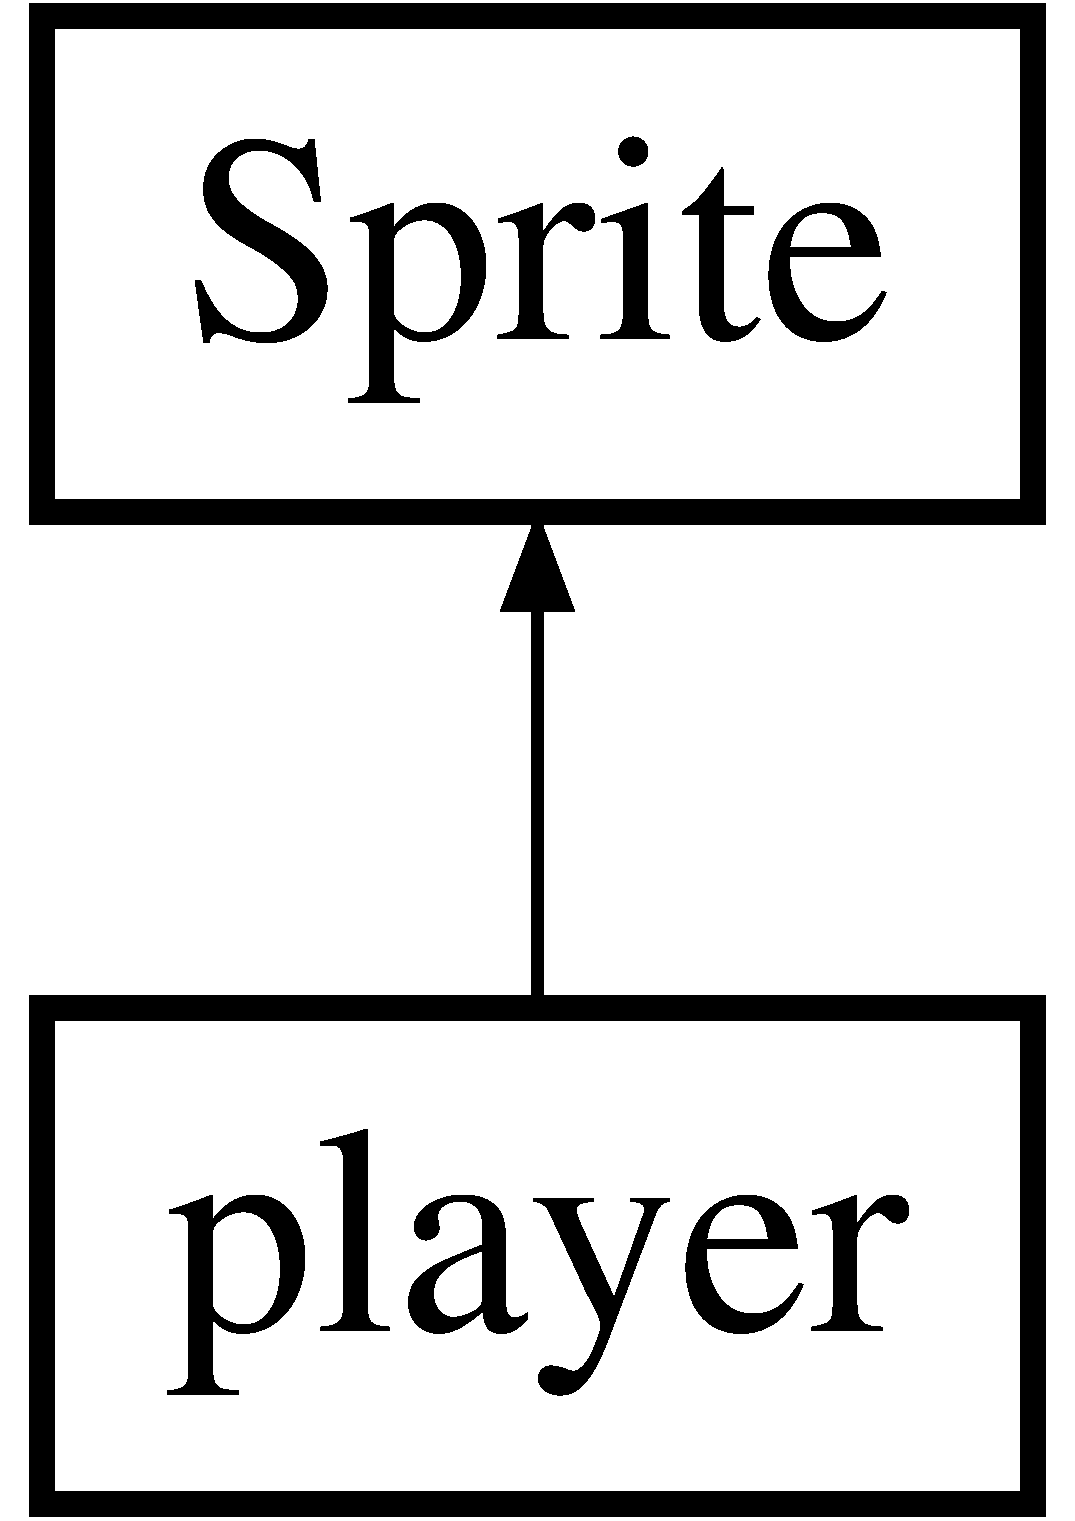
\includegraphics[height=2.000000cm]{classplayer}
\end{center}
\end{figure}
\subsection*{Public Member Functions}
\begin{DoxyCompactItemize}
\item 
\hyperlink{classplayer_a97de83bce15f880241f561b55b016b02}{player} ()
\item 
\hyperlink{classplayer_aab5d2e47b80e0481f09ca0df8b823057}{$\sim$player} ()
\item 
bool \hyperlink{classplayer_a7e688c3070a1d177c5feca760d3c5d58}{get\-Left} () const 
\item 
bool \hyperlink{classplayer_ac7b4b5cf847d851ccb641e878d0ea50d}{get\-Right} () const 
\item 
void \hyperlink{classplayer_a381a5124691a73dd070d2d77bda937ac}{set\-Left} (bool L)
\item 
void \hyperlink{classplayer_a67b3c5f0d7533752b41e4094ac5a1743}{set\-Right} (bool R)
\item 
void \hyperlink{classplayer_a249c3d07b1658c079986646d54dc68f8}{move\-Left} ()
\item 
void \hyperlink{classplayer_aaefc0828be249ecc5a02c5431fda40c5}{move\-Right} ()
\item 
short int \hyperlink{classplayer_a6def826c0e7c2f169c6be74dbcd754b3}{get\-Life} () const 
\item 
void \hyperlink{classplayer_a1e9ab2a4e6896d08cef4a3d96d57bd8d}{lose\-Life} ()
\end{DoxyCompactItemize}


\subsection{Detailed Description}
Player class, this is the pad the player controlls.

here is how it moves and extra life implementation. 

Definition at line 11 of file player.\-h.



\subsection{Constructor \& Destructor Documentation}
\hypertarget{classplayer_a97de83bce15f880241f561b55b016b02}{\index{player@{player}!player@{player}}
\index{player@{player}!player@{player}}
\subsubsection[{player}]{\setlength{\rightskip}{0pt plus 5cm}player\-::player (
\begin{DoxyParamCaption}
{}
\end{DoxyParamCaption}
)}}\label{classplayer_a97de83bce15f880241f561b55b016b02}
default constructor, sets a texture, orgin and position of the player pad. also names how many extra lifes the user has. 

Definition at line 4 of file player.\-cpp.

\hypertarget{classplayer_aab5d2e47b80e0481f09ca0df8b823057}{\index{player@{player}!$\sim$player@{$\sim$player}}
\index{$\sim$player@{$\sim$player}!player@{player}}
\subsubsection[{$\sim$player}]{\setlength{\rightskip}{0pt plus 5cm}player\-::$\sim$player (
\begin{DoxyParamCaption}
{}
\end{DoxyParamCaption}
)}}\label{classplayer_aab5d2e47b80e0481f09ca0df8b823057}


Definition at line 17 of file player.\-cpp.



\subsection{Member Function Documentation}
\hypertarget{classplayer_a7e688c3070a1d177c5feca760d3c5d58}{\index{player@{player}!get\-Left@{get\-Left}}
\index{get\-Left@{get\-Left}!player@{player}}
\subsubsection[{get\-Left}]{\setlength{\rightskip}{0pt plus 5cm}bool player\-::get\-Left (
\begin{DoxyParamCaption}
{}
\end{DoxyParamCaption}
) const}}\label{classplayer_a7e688c3070a1d177c5feca760d3c5d58}
gets the bool value if it should move left. 

Definition at line 43 of file player.\-cpp.

\hypertarget{classplayer_a6def826c0e7c2f169c6be74dbcd754b3}{\index{player@{player}!get\-Life@{get\-Life}}
\index{get\-Life@{get\-Life}!player@{player}}
\subsubsection[{get\-Life}]{\setlength{\rightskip}{0pt plus 5cm}short int player\-::get\-Life (
\begin{DoxyParamCaption}
{}
\end{DoxyParamCaption}
) const}}\label{classplayer_a6def826c0e7c2f169c6be74dbcd754b3}
return have many extra lifes the player has. 

Definition at line 51 of file player.\-cpp.

\hypertarget{classplayer_ac7b4b5cf847d851ccb641e878d0ea50d}{\index{player@{player}!get\-Right@{get\-Right}}
\index{get\-Right@{get\-Right}!player@{player}}
\subsubsection[{get\-Right}]{\setlength{\rightskip}{0pt plus 5cm}bool player\-::get\-Right (
\begin{DoxyParamCaption}
{}
\end{DoxyParamCaption}
) const}}\label{classplayer_ac7b4b5cf847d851ccb641e878d0ea50d}
gets the bool value if it should move right. 

Definition at line 47 of file player.\-cpp.

\hypertarget{classplayer_a1e9ab2a4e6896d08cef4a3d96d57bd8d}{\index{player@{player}!lose\-Life@{lose\-Life}}
\index{lose\-Life@{lose\-Life}!player@{player}}
\subsubsection[{lose\-Life}]{\setlength{\rightskip}{0pt plus 5cm}void player\-::lose\-Life (
\begin{DoxyParamCaption}
{}
\end{DoxyParamCaption}
)}}\label{classplayer_a1e9ab2a4e6896d08cef4a3d96d57bd8d}
decreas the life of the player with 1. 

Definition at line 55 of file player.\-cpp.

\hypertarget{classplayer_a249c3d07b1658c079986646d54dc68f8}{\index{player@{player}!move\-Left@{move\-Left}}
\index{move\-Left@{move\-Left}!player@{player}}
\subsubsection[{move\-Left}]{\setlength{\rightskip}{0pt plus 5cm}void player\-::move\-Left (
\begin{DoxyParamCaption}
{}
\end{DoxyParamCaption}
)}}\label{classplayer_a249c3d07b1658c079986646d54dc68f8}
moves player pad to the left. Has a max see max\-Left for max left value. 

Definition at line 28 of file player.\-cpp.

\hypertarget{classplayer_aaefc0828be249ecc5a02c5431fda40c5}{\index{player@{player}!move\-Right@{move\-Right}}
\index{move\-Right@{move\-Right}!player@{player}}
\subsubsection[{move\-Right}]{\setlength{\rightskip}{0pt plus 5cm}void player\-::move\-Right (
\begin{DoxyParamCaption}
{}
\end{DoxyParamCaption}
)}}\label{classplayer_aaefc0828be249ecc5a02c5431fda40c5}
moves player pad to the right. Has a max see max\-Right for the max right value. 

Definition at line 36 of file player.\-cpp.

\hypertarget{classplayer_a381a5124691a73dd070d2d77bda937ac}{\index{player@{player}!set\-Left@{set\-Left}}
\index{set\-Left@{set\-Left}!player@{player}}
\subsubsection[{set\-Left}]{\setlength{\rightskip}{0pt plus 5cm}void player\-::set\-Left (
\begin{DoxyParamCaption}
\item[{bool}]{L}
\end{DoxyParamCaption}
)}}\label{classplayer_a381a5124691a73dd070d2d77bda937ac}
sets bool value of left move. 

Definition at line 19 of file player.\-cpp.

\hypertarget{classplayer_a67b3c5f0d7533752b41e4094ac5a1743}{\index{player@{player}!set\-Right@{set\-Right}}
\index{set\-Right@{set\-Right}!player@{player}}
\subsubsection[{set\-Right}]{\setlength{\rightskip}{0pt plus 5cm}void player\-::set\-Right (
\begin{DoxyParamCaption}
\item[{bool}]{R}
\end{DoxyParamCaption}
)}}\label{classplayer_a67b3c5f0d7533752b41e4094ac5a1743}
sets bool value of right move. 

Definition at line 23 of file player.\-cpp.



The documentation for this class was generated from the following files\-:\begin{DoxyCompactItemize}
\item 
/home/mejan/\-Documents/skola/\-Cvilingjör\-I\-Datateknik/\-H\-T-\/13/\-Programerings\-\_\-metodiken/\-Projekt/\hyperlink{player_8h}{player.\-h}\item 
/home/mejan/\-Documents/skola/\-Cvilingjör\-I\-Datateknik/\-H\-T-\/13/\-Programerings\-\_\-metodiken/\-Projekt/\hyperlink{player_8cpp}{player.\-cpp}\end{DoxyCompactItemize}

\hypertarget{classsteel_box}{\section{steel\-Box Class Reference}
\label{classsteel_box}\index{steel\-Box@{steel\-Box}}
}


{\ttfamily \#include $<$steel\-Box.\-h$>$}

Inheritance diagram for steel\-Box\-:\begin{figure}[H]
\begin{center}
\leavevmode
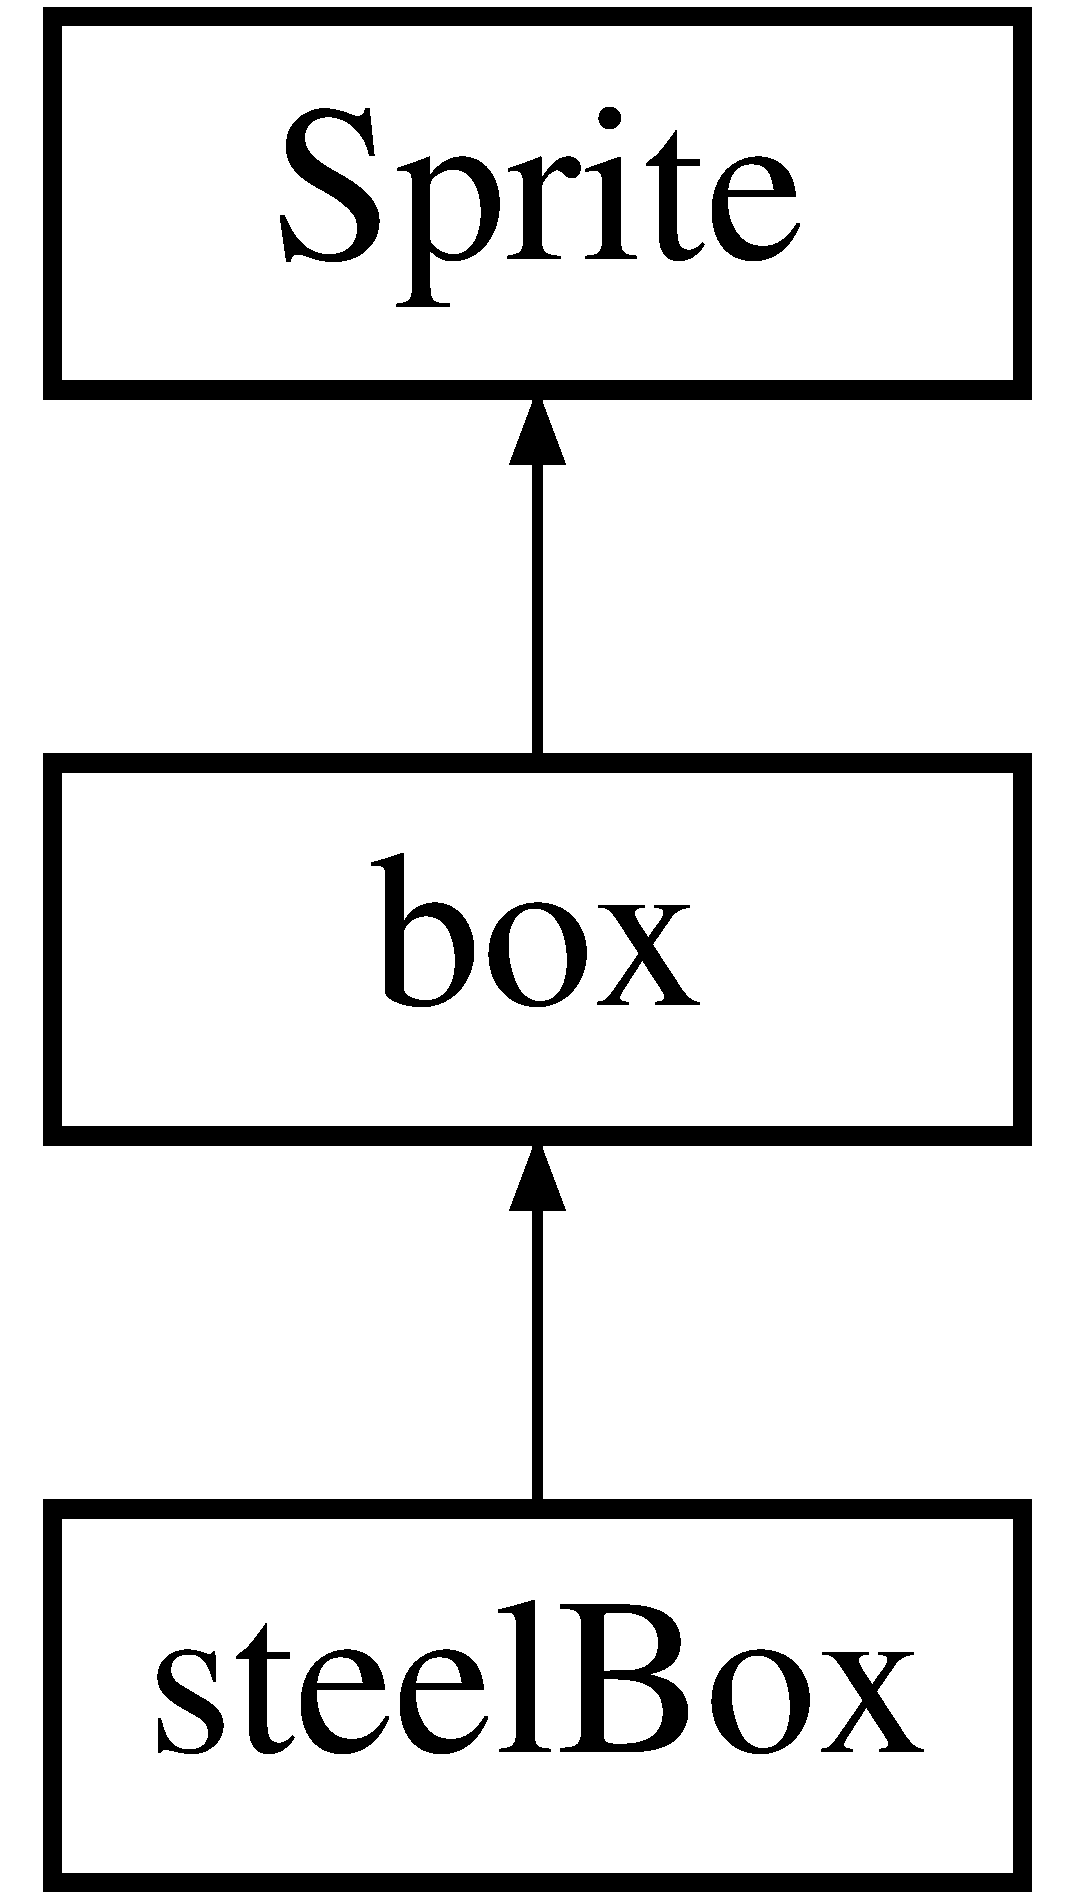
\includegraphics[height=3.000000cm]{classsteel_box}
\end{center}
\end{figure}
\subsection*{Public Member Functions}
\begin{DoxyCompactItemize}
\item 
\hyperlink{classsteel_box_a4516dd36c04ffd32537395a92c60d685}{steel\-Box} ()
\item 
\hyperlink{classsteel_box_ab2444d51a0b52b4131850873ffaddeb1}{$\sim$steel\-Box} ()
\end{DoxyCompactItemize}


\subsection{Detailed Description}


Definition at line 6 of file steel\-Box.\-h.



\subsection{Constructor \& Destructor Documentation}
\hypertarget{classsteel_box_a4516dd36c04ffd32537395a92c60d685}{\index{steel\-Box@{steel\-Box}!steel\-Box@{steel\-Box}}
\index{steel\-Box@{steel\-Box}!steelBox@{steel\-Box}}
\subsubsection[{steel\-Box}]{\setlength{\rightskip}{0pt plus 5cm}steel\-Box\-::steel\-Box (
\begin{DoxyParamCaption}
{}
\end{DoxyParamCaption}
)}}\label{classsteel_box_a4516dd36c04ffd32537395a92c60d685}
uses the box class construct with string and int. string is where it will find the texture the int is the health points this object should have. 

Definition at line 3 of file steel\-Box.\-cpp.

\hypertarget{classsteel_box_ab2444d51a0b52b4131850873ffaddeb1}{\index{steel\-Box@{steel\-Box}!$\sim$steel\-Box@{$\sim$steel\-Box}}
\index{$\sim$steel\-Box@{$\sim$steel\-Box}!steelBox@{steel\-Box}}
\subsubsection[{$\sim$steel\-Box}]{\setlength{\rightskip}{0pt plus 5cm}steel\-Box\-::$\sim$steel\-Box (
\begin{DoxyParamCaption}
{}
\end{DoxyParamCaption}
)}}\label{classsteel_box_ab2444d51a0b52b4131850873ffaddeb1}


Definition at line 5 of file steel\-Box.\-cpp.



The documentation for this class was generated from the following files\-:\begin{DoxyCompactItemize}
\item 
/home/mejan/\-Documents/skola/\-Cvilingjör\-I\-Datateknik/\-H\-T-\/13/\-Programerings\-\_\-metodiken/\-Projekt/\hyperlink{steel_box_8h}{steel\-Box.\-h}\item 
/home/mejan/\-Documents/skola/\-Cvilingjör\-I\-Datateknik/\-H\-T-\/13/\-Programerings\-\_\-metodiken/\-Projekt/\hyperlink{steel_box_8cpp}{steel\-Box.\-cpp}\end{DoxyCompactItemize}

\chapter{File Documentation}
\hypertarget{bounceball_8cpp}{\section{/home/mejan/\-Documents/skola/\-Cvilingjör\-I\-Datateknik/\-H\-T-\/13/\-Programerings\-\_\-metodiken/\-Projekt/bounceball.cpp File Reference}
\label{bounceball_8cpp}\index{/home/mejan/\-Documents/skola/\-Cvilingjör\-I\-Datateknik/\-H\-T-\/13/\-Programerings\-\_\-metodiken/\-Projekt/bounceball.\-cpp@{/home/mejan/\-Documents/skola/\-Cvilingjör\-I\-Datateknik/\-H\-T-\/13/\-Programerings\-\_\-metodiken/\-Projekt/bounceball.\-cpp}}
}
{\ttfamily \#include \char`\"{}bounceball.\-h\char`\"{}}\\*
{\ttfamily \#include $<$random$>$}\\*
{\ttfamily \#include $<$chrono$>$}\\*

\hypertarget{bounceball_8h}{\section{/home/mejan/\-Documents/skola/\-Cvilingjör\-I\-Datateknik/\-H\-T-\/13/\-Programerings\-\_\-metodiken/\-Projekt/bounceball.h File Reference}
\label{bounceball_8h}\index{/home/mejan/\-Documents/skola/\-Cvilingjör\-I\-Datateknik/\-H\-T-\/13/\-Programerings\-\_\-metodiken/\-Projekt/bounceball.\-h@{/home/mejan/\-Documents/skola/\-Cvilingjör\-I\-Datateknik/\-H\-T-\/13/\-Programerings\-\_\-metodiken/\-Projekt/bounceball.\-h}}
}
{\ttfamily \#include $<$S\-F\-M\-L/\-Graphics.\-hpp$>$}\\*
{\ttfamily \#include $<$iostream$>$}\\*
{\ttfamily \#include $<$math.\-h$>$}\\*
\subsection*{Classes}
\begin{DoxyCompactItemize}
\item 
class \hyperlink{classbounce_ball}{bounce\-Ball}
\end{DoxyCompactItemize}

\hypertarget{box_8cpp}{\section{/home/mejan/\-Documents/skola/\-Cvilingjör\-I\-Datateknik/\-H\-T-\/13/\-Programerings\-\_\-metodiken/\-Projekt/box.cpp File Reference}
\label{box_8cpp}\index{/home/mejan/\-Documents/skola/\-Cvilingjör\-I\-Datateknik/\-H\-T-\/13/\-Programerings\-\_\-metodiken/\-Projekt/box.\-cpp@{/home/mejan/\-Documents/skola/\-Cvilingjör\-I\-Datateknik/\-H\-T-\/13/\-Programerings\-\_\-metodiken/\-Projekt/box.\-cpp}}
}
{\ttfamily \#include \char`\"{}box.\-h\char`\"{}}\\*

\hypertarget{box_8h}{\section{/home/mejan/\-Documents/skola/\-Cvilingjör\-I\-Datateknik/\-H\-T-\/13/\-Programerings\-\_\-metodiken/\-Projekt/box.h File Reference}
\label{box_8h}\index{/home/mejan/\-Documents/skola/\-Cvilingjör\-I\-Datateknik/\-H\-T-\/13/\-Programerings\-\_\-metodiken/\-Projekt/box.\-h@{/home/mejan/\-Documents/skola/\-Cvilingjör\-I\-Datateknik/\-H\-T-\/13/\-Programerings\-\_\-metodiken/\-Projekt/box.\-h}}
}
{\ttfamily \#include $<$S\-F\-M\-L/\-Graphics.\-hpp$>$}\\*
{\ttfamily \#include $<$string$>$}\\*
{\ttfamily \#include $<$iostream$>$}\\*
\subsection*{Classes}
\begin{DoxyCompactItemize}
\item 
class \hyperlink{classbox}{box}
\end{DoxyCompactItemize}

\hypertarget{game_8cpp}{\section{/home/mejan/\-Documents/skola/\-Cvilingjör\-I\-Datateknik/\-H\-T-\/13/\-Programerings\-\_\-metodiken/\-Projekt/game.cpp File Reference}
\label{game_8cpp}\index{/home/mejan/\-Documents/skola/\-Cvilingjör\-I\-Datateknik/\-H\-T-\/13/\-Programerings\-\_\-metodiken/\-Projekt/game.\-cpp@{/home/mejan/\-Documents/skola/\-Cvilingjör\-I\-Datateknik/\-H\-T-\/13/\-Programerings\-\_\-metodiken/\-Projekt/game.\-cpp}}
}
{\ttfamily \#include \char`\"{}game.\-h\char`\"{}}\\*

\hypertarget{game_8h}{\section{/home/mejan/\-Documents/skola/\-Cvilingjör\-I\-Datateknik/\-H\-T-\/13/\-Programerings\-\_\-metodiken/\-Projekt/game.h File Reference}
\label{game_8h}\index{/home/mejan/\-Documents/skola/\-Cvilingjör\-I\-Datateknik/\-H\-T-\/13/\-Programerings\-\_\-metodiken/\-Projekt/game.\-h@{/home/mejan/\-Documents/skola/\-Cvilingjör\-I\-Datateknik/\-H\-T-\/13/\-Programerings\-\_\-metodiken/\-Projekt/game.\-h}}
}
{\ttfamily \#include \char`\"{}steel\-Box.\-h\char`\"{}}\\*
{\ttfamily \#include \char`\"{}player.\-h\char`\"{}}\\*
{\ttfamily \#include \char`\"{}bounceball.\-h\char`\"{}}\\*
{\ttfamily \#include \char`\"{}gui.\-h\char`\"{}}\\*
{\ttfamily \#include $<$vector$>$}\\*
{\ttfamily \#include $<$cstdlib$>$}\\*
{\ttfamily \#include $<$math.\-h$>$}\\*
{\ttfamily \#include $<$sstream$>$}\\*
\subsection*{Classes}
\begin{DoxyCompactItemize}
\item 
class \hyperlink{classgame}{game}
\end{DoxyCompactItemize}

\hypertarget{gui_8cpp}{\section{/home/mejan/\-Documents/skola/\-Cvilingjör\-I\-Datateknik/\-H\-T-\/13/\-Programerings\-\_\-metodiken/\-Projekt/gui.cpp File Reference}
\label{gui_8cpp}\index{/home/mejan/\-Documents/skola/\-Cvilingjör\-I\-Datateknik/\-H\-T-\/13/\-Programerings\-\_\-metodiken/\-Projekt/gui.\-cpp@{/home/mejan/\-Documents/skola/\-Cvilingjör\-I\-Datateknik/\-H\-T-\/13/\-Programerings\-\_\-metodiken/\-Projekt/gui.\-cpp}}
}
{\ttfamily \#include \char`\"{}gui.\-h\char`\"{}}\\*

\hypertarget{gui_8h}{\section{/home/mejan/\-Documents/skola/\-Cvilingjör\-I\-Datateknik/\-H\-T-\/13/\-Programerings\-\_\-metodiken/\-Projekt/gui.h File Reference}
\label{gui_8h}\index{/home/mejan/\-Documents/skola/\-Cvilingjör\-I\-Datateknik/\-H\-T-\/13/\-Programerings\-\_\-metodiken/\-Projekt/gui.\-h@{/home/mejan/\-Documents/skola/\-Cvilingjör\-I\-Datateknik/\-H\-T-\/13/\-Programerings\-\_\-metodiken/\-Projekt/gui.\-h}}
}
{\ttfamily \#include $<$S\-F\-M\-L/\-Graphics.\-hpp$>$}\\*
{\ttfamily \#include $<$iostream$>$}\\*
\subsection*{Classes}
\begin{DoxyCompactItemize}
\item 
class \hyperlink{classgui}{gui}
\end{DoxyCompactItemize}

\hypertarget{main_8cpp}{\section{/home/mejan/\-Documents/skola/\-Cvilingjör\-I\-Datateknik/\-H\-T-\/13/\-Programerings\-\_\-metodiken/\-Projekt/main.cpp File Reference}
\label{main_8cpp}\index{/home/mejan/\-Documents/skola/\-Cvilingjör\-I\-Datateknik/\-H\-T-\/13/\-Programerings\-\_\-metodiken/\-Projekt/main.\-cpp@{/home/mejan/\-Documents/skola/\-Cvilingjör\-I\-Datateknik/\-H\-T-\/13/\-Programerings\-\_\-metodiken/\-Projekt/main.\-cpp}}
}
{\ttfamily \#include \char`\"{}game.\-h\char`\"{}}\\*
{\ttfamily \#include $<$iostream$>$}\\*
{\ttfamily \#include $<$sstream$>$}\\*
\subsection*{Functions}
\begin{DoxyCompactItemize}
\item 
int \hyperlink{main_8cpp_ae66f6b31b5ad750f1fe042a706a4e3d4}{main} ()
\end{DoxyCompactItemize}


\subsection{Function Documentation}
\hypertarget{main_8cpp_ae66f6b31b5ad750f1fe042a706a4e3d4}{\index{main.\-cpp@{main.\-cpp}!main@{main}}
\index{main@{main}!main.cpp@{main.\-cpp}}
\subsubsection[{main}]{\setlength{\rightskip}{0pt plus 5cm}int main (
\begin{DoxyParamCaption}
{}
\end{DoxyParamCaption}
)}}\label{main_8cpp_ae66f6b31b5ad750f1fe042a706a4e3d4}
Mikael Falk \href{mailto:mifa1100@student.miun.se}{\tt mifa1100@student.\-miun.\-se}

This is a simpel break out game main just calls the class constructor for game. 

Definition at line 13 of file main.\-cpp.


\hypertarget{player_8cpp}{\section{/home/mejan/\-Documents/skola/\-Cvilingjör\-I\-Datateknik/\-H\-T-\/13/\-Programerings\-\_\-metodiken/\-Projekt/player.cpp File Reference}
\label{player_8cpp}\index{/home/mejan/\-Documents/skola/\-Cvilingjör\-I\-Datateknik/\-H\-T-\/13/\-Programerings\-\_\-metodiken/\-Projekt/player.\-cpp@{/home/mejan/\-Documents/skola/\-Cvilingjör\-I\-Datateknik/\-H\-T-\/13/\-Programerings\-\_\-metodiken/\-Projekt/player.\-cpp}}
}
{\ttfamily \#include \char`\"{}player.\-h\char`\"{}}\\*

\hypertarget{player_8h}{\section{/home/mejan/\-Documents/skola/\-Cvilingjör\-I\-Datateknik/\-H\-T-\/13/\-Programerings\-\_\-metodiken/\-Projekt/player.h File Reference}
\label{player_8h}\index{/home/mejan/\-Documents/skola/\-Cvilingjör\-I\-Datateknik/\-H\-T-\/13/\-Programerings\-\_\-metodiken/\-Projekt/player.\-h@{/home/mejan/\-Documents/skola/\-Cvilingjör\-I\-Datateknik/\-H\-T-\/13/\-Programerings\-\_\-metodiken/\-Projekt/player.\-h}}
}
{\ttfamily \#include $<$S\-F\-M\-L/\-Graphics.\-hpp$>$}\\*
{\ttfamily \#include $<$iostream$>$}\\*
\subsection*{Classes}
\begin{DoxyCompactItemize}
\item 
class \hyperlink{classplayer}{player}
\end{DoxyCompactItemize}

\hypertarget{steel_box_8cpp}{\section{/home/mejan/\-Documents/skola/\-Cvilingjör\-I\-Datateknik/\-H\-T-\/13/\-Programerings\-\_\-metodiken/\-Projekt/steel\-Box.cpp File Reference}
\label{steel_box_8cpp}\index{/home/mejan/\-Documents/skola/\-Cvilingjör\-I\-Datateknik/\-H\-T-\/13/\-Programerings\-\_\-metodiken/\-Projekt/steel\-Box.\-cpp@{/home/mejan/\-Documents/skola/\-Cvilingjör\-I\-Datateknik/\-H\-T-\/13/\-Programerings\-\_\-metodiken/\-Projekt/steel\-Box.\-cpp}}
}
{\ttfamily \#include \char`\"{}steel\-Box.\-h\char`\"{}}\\*

\hypertarget{steel_box_8h}{\section{/home/mejan/\-Documents/skola/\-Cvilingjör\-I\-Datateknik/\-H\-T-\/13/\-Programerings\-\_\-metodiken/\-Projekt/steel\-Box.h File Reference}
\label{steel_box_8h}\index{/home/mejan/\-Documents/skola/\-Cvilingjör\-I\-Datateknik/\-H\-T-\/13/\-Programerings\-\_\-metodiken/\-Projekt/steel\-Box.\-h@{/home/mejan/\-Documents/skola/\-Cvilingjör\-I\-Datateknik/\-H\-T-\/13/\-Programerings\-\_\-metodiken/\-Projekt/steel\-Box.\-h}}
}
{\ttfamily \#include \char`\"{}box.\-h\char`\"{}}\\*
\subsection*{Classes}
\begin{DoxyCompactItemize}
\item 
class \hyperlink{classsteel_box}{steel\-Box}
\end{DoxyCompactItemize}

%--- End generated contents ---

% Index
\newpage
\phantomsection
\addcontentsline{toc}{chapter}{Index}
\printindex

\end{document}
